\chapter{Resultados Experimentais} \label{chap:resexp}


Os testes desta secção têm como objetivo encontrar o melhor detetor / descritor / matcher , determinando a robustez do subsistema de localização para o ruído, iluminação variante e rotação.

Os parâmetros utilizados nos vários detetores para limitar o número de pontos característicos são definidos com base no valor médio de intensidade da imagem. Desta forma, os detetores trabalham sob várias condições de brilho.

Para obter resultados constantes, a plataforma ROS permite ao usuário reproduzir uma sequência de mensagens nas mesmas condições em que foram adquiridas. Esta funcionalidade permite ao desenvolvedor resultados constantes, ou seja, diferentes combinações de parâmetros podem ser testadas para a mesma entrada exata.

\section{Calibração da câmara}

Como mencionado anteirormente, no capítulo ~\ref{section:Intrin}, as câmara e lente têm que ser calibrada para não causar erros de distorção nos resultados finais. 

\begin{figure}[h!]  %colocar figura a seguir ao texto anterior
	\centering
	\includegraphics[width=0.4\linewidth]{checkboard.png} 
	\caption{Quadrado de xadrez para calibrar câmara.}
	\label{fig:checkboard}  %30 years. Figure 3 a)
\end{figure}

Desta forma, é usado o algoritmo desenvolvido em ~\cite{piCam}. O algoritmo baseia-se no uso de um quadrado de xadrez , figura ~\ref{fig:checkboard}. Este é composto por quadrados com a mesma largura e devido à sua composição em xadrez é fácil a determinação de pontos de intreseção \ cruzamento. Com estes pontos é possivel criar linhas com tamanhos conhecidos e através destas obter os parâmetros intrinsecos da camâra e lente. 



A figura ~\ref{fig:imgcheckboard} ilustra a calibração da devida câmara do raspberry pi com uma lente olho de peixe \textit{full-frame}. O resultado final é a matriz de parâmetros intrinsecos composta por : \[ \left[ \begin{array}{ccc}
306.442 & 0 & 330.165 \\ 
0 & 306.27 & 234.44 \\ 
0 & 0 & 1
\end{array} \right] \] e matriz de parâmetros de distorção \[ \left[\begin{array}{ccccc}
-0.27 & 0.0445 & 0.000077 & 0.000007 & 0 
\end{array} \right] \]

\begin{figure}[h!]  %colocar figura a seguir ao texto anterior
	\centering
	\includegraphics[width=0.6\linewidth]{imgcheckboard.png} 
	\caption{Imagem da calibração dos parâmetros da câmara.}
	\label{fig:imgcheckboard}  %30 years. Figure 3 a)
\end{figure}


\section{Diferença entre detetores de características}

Nesta dissertação serão comparados 4 detetores de características, explicitos em  ~\ref{detCar}. Os testes são realizados num ambiente agrícola para maior coerência com o objectivo da dissertação, como ilustrado na figura ~\ref{fig:4metodos}.


\begin{figure}[h!]  %colocar figura a seguir ao texto anterior
	\begin{center}
	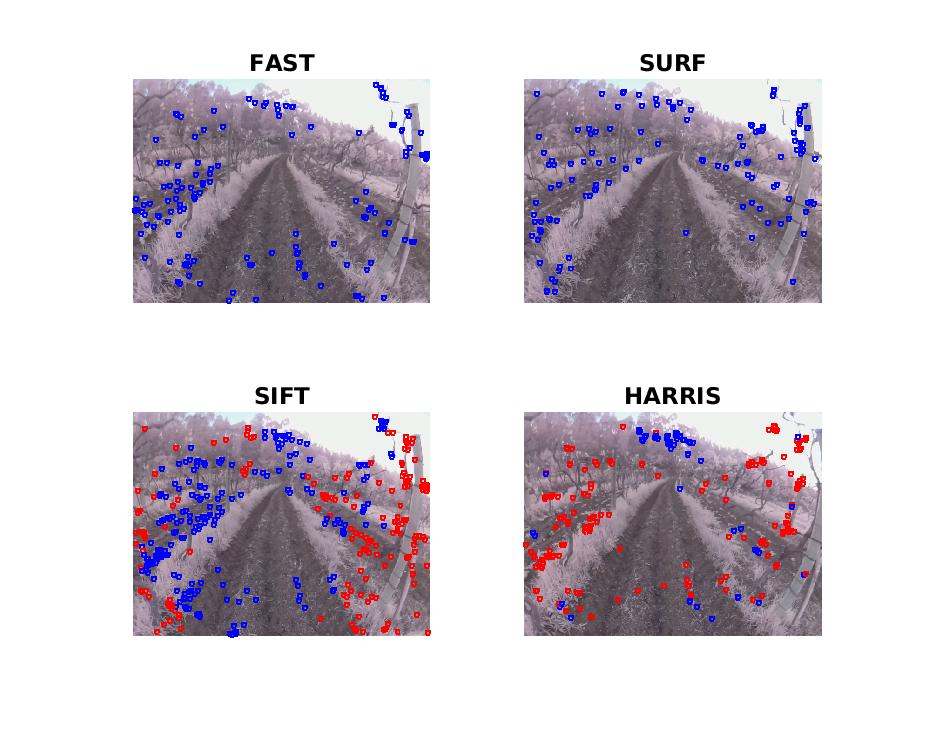
\includegraphics[width=0.8\linewidth]{FAST_SURF_SIFT_HARRIS.eps} 
	\caption{Distribuição dos pontos caracterisiticos para os quatro detetores de características, FAST , SURF, SIFT, HARRIS.}
	\label{fig:4metodos}  %30 years. Figure 3 a)
	\end{center}
\end{figure}


De notar que os pontos azuis são pontos de caracteristicas que têm correspondências corretas no próximo frame e os pontos vermelhos são \textit{outliers}, pontos com correspondência de caracteristicas erradas e/ou sem correspondências.

Os métodos têm as sua diferenças, desde logo a quantidade dos pontos com correspondência no frame seguinte. Desta forma, o método HARRIS é péssimo, devido às poucas correspondências, e o método SIFT discarta muitos pontos característicos de curta distância. A distribuição dos pontos caracteristicos é favoravél no método SURF , FAST e SIFT, sendo o primeiro o melhor, com maior seleção dos pontos na videiras, sendo estes mais estáveis e recomendados devido ao ambiente vinicula. Em termos de quantidade de pontos o método SIFT têm demasiados o que implica em maior tempo de processamento e maior número de frames perdidos entre processamento. Esta quantidade podia ser diminuida mas em cenários 
mais precários o algoritmo fica sujeito a encontrar um numero reduzido de pontos caracteristicos que impossibilitem o fucnionamento do algortimo. 

Assim, o método HARRIS é o pior devido a fraca qualidade e distribuição dos pontos caracteristicos. O método SIFT tem um grande tempo de processamento que caso a velocidade do robô seja baixa é uma solução plausivel devido a boa quantidade de pontos caracteristicos e boa distribuição. Por fim, o método FAST e SURF são os mais indicativos. Sendo, o último com melhor distribuição  dos pontos caracteristicos. 


\section{Testes}

De forma a validar o algoritmo de localização os testes requerem a quantificação do erro. O erro é descrito com a diferença entre o valor real e o valor medido.

As coordenadas reais têm de ser obtidas através de um sensor externo, tal como a laser baseado em localização, odometria das rodas or mesmo uma fita métrica. \textbf{\textit{Devido ao declive dos terrenos e estrutura é utilizada uma fita métrica para comparação dos resultados.}}

Os devidos testes foram realizados em ambiente agrícola, precisamente numa vinha. Os percursos efetuados foram : estático, movimento em linha reta, movimento em L (semi-quadrado), percurso quadrangular, percurso retangular e percurso circular. De notar que os percursos foram realizados com velocidades baixas. Assim, a câmara consegue extrair um maior número de características e por consequência o erro da trajetória estimada será menor.  


\subsection{Teste de parâmetros}

Quatro parâmetros foram escolhidos para comparar a combinação dos detetores / descritores e matchers. Eles são :

\begin{itemize}
	\item \textbf{Imagens processadas} - Corresponde ao número de imagens que o programa conseguiu processar. É proporcional à velocidade do ciclo de processamento.
	\item \textbf{Média de frames perdidos} - Quantidade de frames perdidos entre ciclos.
	\item \textbf{Média matches por imagem} - Corresponde à média de correspondências encontradas para cada imagem depois de filtrar outliers.
	\item \textbf{Média de processamento} - Corresponde à média da duração de processamento de ciclo.
\end{itemize}


\subsection{Sequência sem Movimento}

Devido à fita métrica não produzir medidas em tempo real do movimento, o primeiro teste é feito com uma sequência de frames, or bags, onde o robô não se movimenta.

\subsection{Deteção da trajetória}

\textit{\textbf{
Devido ao erro deste teste não poder ser quantificado, este serve apenas como demonstração ou provas de conceito. A validação do resultado é visual.}}

